\documentclass{bigdata}
\usepackage[utf8]{inputenc}
\DeclareMathOperator*{\argmax}{arg\,max}
\DeclareMathOperator*{\argmin}{arg\,min}

\title{Multimedia Retrieval}
\author{Diego Renders}
\date{Oktober 2019}


\begin{document}
\maketitle

\section{Introduction}

\paragraph*{Problem statement.}

\newpage

\section{Frequent item set mining}

At various points we discussed frequent item set mining. Do not make this section a large list of definitions and facts. A common mistake is that a student constricts this dissertation to only contain a list of facts: ``a \emph{lattice} is a structure with three properties: \emph{idempotency}, \emph{commutativity}, \emph{associativity} - (end of section)''. It is O.K. to spend time on discussing properties, but focus on the following: what power do these definitions give you? What is the purpose of a property like commutativity? You can also provide examples of where these properties occur in data.

Another common mistake is that a student only focuses on the formal (mathematical) definitions surrounding item set mining. e.g.: ``We say that there is a \emph{Galois connection} between two lattices $(P(\mathcal{I}, \subseteq)$ and $P(\mathcal{D}, \subseteq)$ if for $I \in P(\mathcal{I}, \subseteq)$ and $E' \in P(\mathcal{D}, \subseteq)$ we have that (Lecture 3, slide 31):'' 

\begin{align*}
    \left[    E' \subseteq F(I)    \right] \Leftrightarrow \left[  \forall t \in E' \mid I \subseteq t   \right] \\
    \Leftrightarrow    \left[ I \subseteq \cap_{t \in E'} t    \right] \Leftrightarrow \left[ I \subseteq  G(E')  \right]
\end{align*}

However, this only demonstrates that you are able to copy a definition from a slide. \underline{If} you decide to discuss a property such as a Galois connection, then describe the semantics of the definition and focus on what each a property is good for: what kind of problem is this property trying to solve or circumvent? 

This section is at most one-and-a-half page. Below is a list of terms that you should mention. Whenever you mention a definition, always focus on the intuition behind the definition and on what ``power'' the definition gives you.

\begin{itemize}
    \item Transactional databases.
    \item Frequent items sets.
    \item (Optional) You could be more general and describe frequent patterns.
    \item Apriori.
    \item Closures.
    \item Range spaces of frequent item sets.
    \item From frequent item set mining to classification.
\end{itemize}




\section{Part 1}

\subsection{Database evaluation}
The database contains around 1800 models in off file format. All of the models contain only triangles as faces. The distribution of faces is shown in figure ?. The average number of vertices is 4221, the minimum 10, and the maximum 160940. The histogram, along with the average, shows that most of the models have a vertex count of smaller than twenty thousand. In order to successfully perform the upcoming steps of feature extraction the models need to have approximately the same number of vertices. Two actions can be undertaken to achieve this, supersampling and subsampling. Supersample the models with a low vertex count, and subsample the models with a large vertex count. A target number of vertices has to be chosen for this. One solution could be to choose the average. However because several of the meshes have a very high resolution of a hundred thousand vertices, subsampling this to reach the four thousand required vertices would ruin the original shape. Therefore the target vertices is chosen to be higher than the average, so that the higher resolution models retain their characteristics. The only downside for choosing a higher target number of vertices is an increase in computation time. The target number of vertices is set at forty thousand, the methodology for supersampling and subsampling is explained in the following two sections.

\begin{figure}[h!]
  \centering
    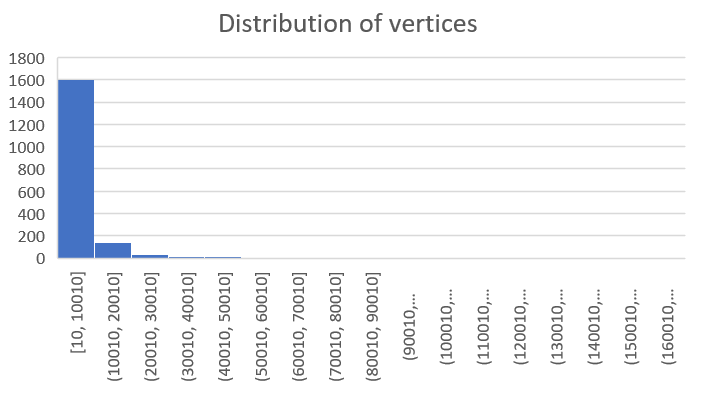
\includegraphics[width=\linewidth]{Pictures/verticesHist.png}
    \caption{Histogram showing the distribution of vertices in the PSB database}
\end{figure}

\subsection{Supersampling}

\subsection{Subsampling}
For the task of subsampling the Polygon Mesh Processing (pmp) library is used. The SurfaceSimplification class is used to perform mesh decimation, taking as input the mesh and a target number of vertices. To demonstrate that this algorithm works correctly for our models a pre and post visualisation is shown in figure 2. This is the largest model in the dataset with 316.498 faces and 160.940 vertices. The post decimation model contains 78.473 faces and 40.000 vertices. Even though the model only has a fourth of its original vertices, it clearly retains its characteristics. Therefore we can conclude that the algorithm is a suitable tool for this project.

\begin{figure}[h!]
  \centering
  \begin{subfigure}[b]{0.4\linewidth}
    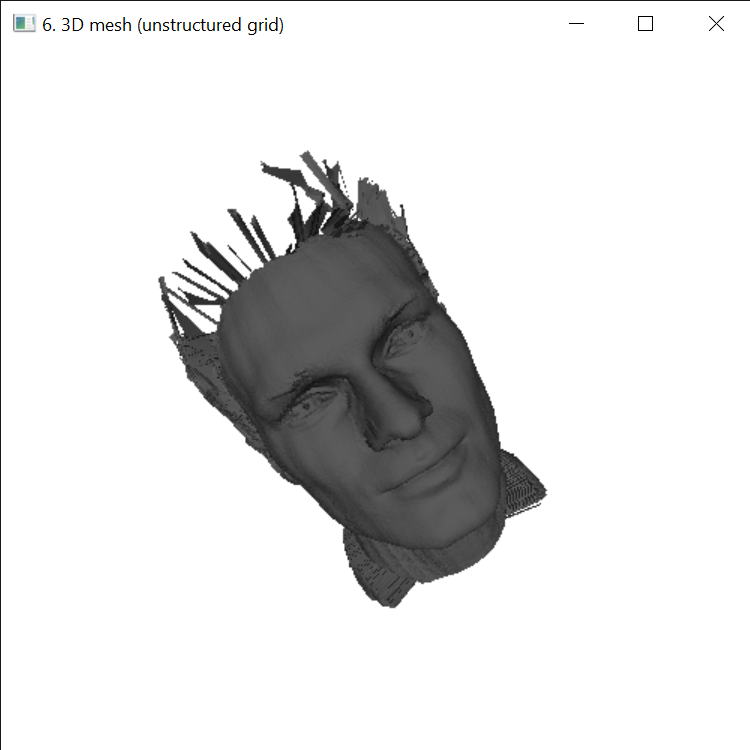
\includegraphics[width=\linewidth]{Pictures/preSub.png}
    \caption{Pre decimation}
  \end{subfigure}
  \begin{subfigure}[b]{0.4\linewidth}
    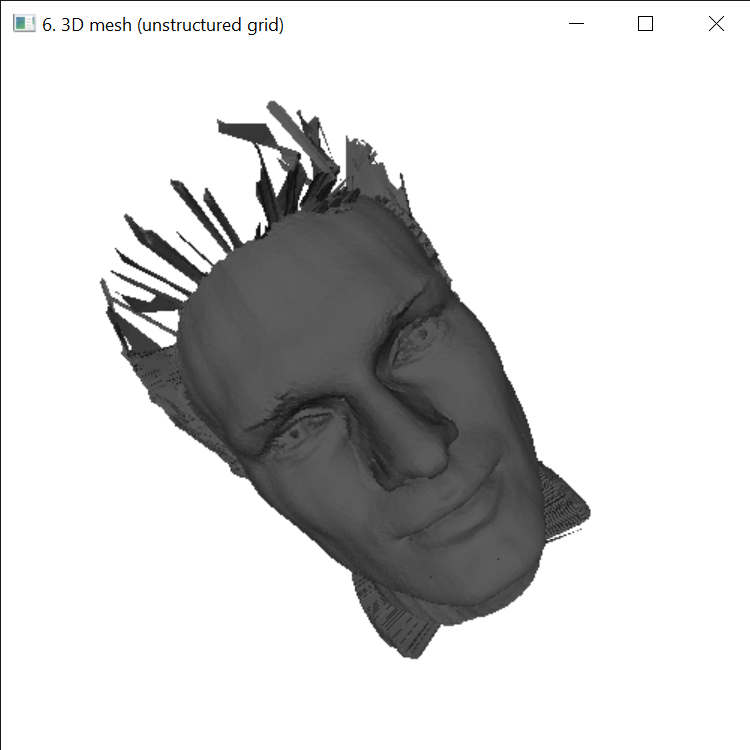
\includegraphics[width=\linewidth]{Pictures/postSub.png}
    \caption{Post decimation}
  \end{subfigure}
  \caption{Model m303 before and after mesh decimation}
  \label{fig:decimatedMesh}
\end{figure}

\subsection{Four step normalization}

Next each mesh will go through the four step normalization pipeline so that it is ready to be used in upcoming tasks. Figure 1 shows a visualization of what each step does, the red, green, and blue represent the $x$, $y$, and $z$ axises respectively from zero to one. The first step is to center on the Barycenter, than in step 2 PCA is done to orient the object in an intuitive way. Step 3 performs a fliptest which result in the majority of the mass in the object to be located in the negative side of the axis. Finally step 4 normalizes the model, which is excluded in the figure because the model was already normalized and thus would show no difference.

\begin{figure}[h!]
  \centering
  \begin{subfigure}[b]{0.4\linewidth}
    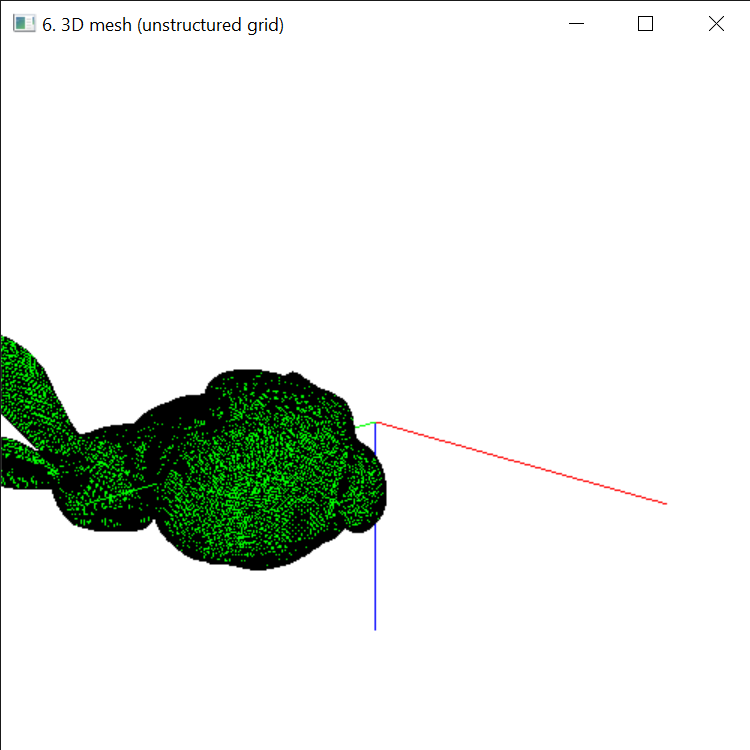
\includegraphics[width=\linewidth]{Pictures/Part2/Step0.png}
    \caption{Step 0}
  \end{subfigure}
  \begin{subfigure}[b]{0.4\linewidth}
    \includegraphics[width=\linewidth]{Pictures/Part2/step1.png}
    \caption{Step 1 Barycenter}
  \end{subfigure}
  \begin{subfigure}[b]{0.4\linewidth}
    \includegraphics[width=\linewidth]{Pictures/Part2/step2.png}
    \caption{Step 2 PCA}
  \end{subfigure}
  \begin{subfigure}[b]{0.4\linewidth}
    \includegraphics[width=\linewidth]{Pictures/Part2/step3.png}
    \caption{Step 3 Fliptest}
  \end{subfigure}
  \caption{Visualization of the Four step normalization pipeline.}
  \label{fig:bunny}
\end{figure}

\subsection{Step 1. Center on the barycenter}

For the first step the barycenter $b$ is calculated, which is the average x, y, and z coordinates of all vertices in the mesh. Next, each vertex $v$ is translated, by subtracting these averages from each of its points resulting in the new vertex position $u$.
\[
\begin{bmatrix}
u_x \\
u_y \\
u_z \\
\end{bmatrix}
=
\begin{bmatrix}
v_x \\
v_y \\
v_z \\
\end{bmatrix}
-
\begin{bmatrix}
b_x \\
b_y \\
b_z \\
\end{bmatrix}
\]

The result can be verified by calculating the average coordinates again, which should be 0 after the normalization.

\subsection{Step 2. PCA}
Prinicipal component analysis is done using the arglib library. The three eigenvectors $e_1$, $e_2$, and $e_3$ are returned by the algorithm. A translation matrix M is than created using the vectors $x$, $y$, and $z$, that represent the axises of the normal coordinate system.

\[
x = 
\begin{bmatrix}
1 \\
0 \\
0 \\
\end{bmatrix}
y =
\begin{bmatrix}
0 \\
1 \\
0 \\
\end{bmatrix}
z =
\begin{bmatrix}
0 \\
0 \\
1 \\
\end{bmatrix}
M =
\begin{bmatrix}
x \cdot e_1 & x \cdot e_2 & x \cdot e_3 \\
y \cdot e_1 & y \cdot e_2 & y \cdot e_3 \\
z \cdot e_1 & z \cdot e_2 & z \cdot e_3 \\
\end{bmatrix}
\]

The new vertex $u$ is obtained by multiplying this matrix with the old vertex $v$.

\[
\begin{bmatrix}
u_x \\
u_y \\
u_z \\
\end{bmatrix}
=
M
\cdot
\begin{bmatrix}
v_x \\
v_y \\
v_z \\
\end{bmatrix}
\]

The result of the translation can easily be verified. Doing PCA again on the translated mesh returns three eigenvectors that now correspond with the $x$, $y$, and $z$ axis.

\subsection{Step 3. Fliptest}
The eigenvectors used for the translation in the previous step are unoriented and thus give no information about to which side the model should be directed. Using the fliptest it is ensured that the majority of the mass resides in the negative half-space. Mass in this case is not indicated by the number of the vertices but also takes momentum into consideration, i.e. vertices farther away from the origin have a higher weight. Three variables are introduced: $w_x$, $w_y$, and $w_z$ that indicate the total weight of each of three coordinates. 
\begin{equation}
w_i = \sum sign(C_{t,i})(C_{t,i})^2
\end{equation}
 where $C_{t,i}$ is the $i^{th}$ coordinate of triangle t ($i \in {x,y,z}$). The latter part of the summation gives coordinates far away from the origin an higher weight, while the former part gives it either a negative or positive weight. These values are than used for a new translation matrix $M$. Which flips the coordinates if necessary, in case the mesh is already properly oriented $M$ will simply be the identity matrix.
\[
M = 
\begin{bmatrix}
sign(w_x) & 0 & 0 \\
0 & sign(w_y) & 0 \\
0 & 0 & sign(w_z) \\
\end{bmatrix}
\]

\subsection{Step 4. Normalization}
The last step scales the model in the unit volume, i.e. it can fit in a unit cube. First the min and max of the $x$,$y$, and $z$ coordinates of the axis-aligned bounding box is found. Next the largest distance $\delta$ between the min and max of these coordinates is used for the scaling factor $s = \frac{1}{\delta}$. Finally each vertex $v$ is multiplied with this factor to obtain the new vertex $u$.

\[
\begin{bmatrix}
u_x \\
u_y \\
u_z \\
\end{bmatrix}
=
\begin{bmatrix}
v_x \\
v_y \\
v_z \\
\end{bmatrix}
\cdot s
\]

A visualization is excluded, however the effectiveness of this step can easily be verified by looking at the resulting bounding box of the model.

\newpage

\section{Frequent item set mining on big data}

This course aims to explain the results from two influential papers (Toivonen 1996, Riondato and Upfal 2014) on the subject of frequent item set mining. In this section, you demonstrate your knowledge of the course by describing both results and by discussing the difference between the two results. All the relevant content for this section was covered during the course, there is no need to read the two papers. 

The previous sections are designed to contain all the definitions, prior results and concepts that are needed to understand the result from Toivonen and Riondato and Upfal. Hence, this section can be rather short. Each subsection should be at most half a page.



\subsection{Toivonen and frequent item sets}

Toivonen was one of the first to describe how to find frequent item sets on big data sets. Specifically, Toivonen specifies how large a sample should be, before you can ``accurately'' learn frequent item sets from a large database. In this subsection you should discuss this theoretical result.

\subsection{PAC-learning and frequent item sets}

Riondato and Upfal showed that the problem of frequent item set mining is PAC-learnable. This subsection should discuss two things:
Why is it possible to PAC-learn frequent item sets and how large should your sample size be (according to Riondato and Upfal) and \underline{why}? Refer to explanations and definitions from prior sections such as range spaces.

\subsection{Toivonen vs PAC-learning}

We have seen two approaches for sampling for frequent item set mining which gives us two different bounds for the sample size, and different assurances for each result.
In this subsection you should discuss what these differences are.


\section{Mandatory extra section}

The main goal of this course is to explain the two mentioned influential big data papers. In the previous sections you demonstrate your knowledge of basic concepts of data mining and you showed your understanding of the theoretical sampling bounds by Toivonen, Riondato and Upfal. We hope, that these topics form a solid basis for knowledge and that your understanding of these topics allows you to acquire new knowledge around big data on your own. 

In the extra section, you must choose one out of four possible topics, and supply us with information which is not covered in the main part of the course. However, on each topic there was at least one lecture! Just as in the rest of the essay, we want you to focus not on definitions and factual information, but on concepts and understanding. The extra section should be 1 page. The four topics are ordered on difficulty, with the last topic being the most difficult. More ambitious students, receive more ambitious grades but remember that we would rather see a good dissertation on a normal topic over a poor dissertation on a difficult topic! The four topics are:

\begin{enumerate}
    \item Bootstrapping and missing data.
    \item Structural Risk minimization.
    \item Adaptive Boosting (adaboost).
    \item Bounds on the VC-dimension.
\end{enumerate}

\begin{figure}[t]
  \centering
  \caption{Student 1 is a regular student aiming for a sufficient. Student 1 filled every section up to the maximal limit and then wrote an extra section about a less-ambitious topic of exactly one page.}
    \label{fig:student1}
\end{figure}


We expect that you discuss this new information on the same theoretical level of depth as the rest of this course. For each of these four topics, there exist hard theoretical guarantees. Try to discuss one of these theoretical results or guarantees. \underline{Do not} describe a long list of often used techniques with only citations. There is an example of an extra section below.

\section{Useful information:}

Here is some useful information for if you want to get started on your essay. This section should be especially useful if you make it in LaTeX.
Here is how you include a figure and reference to a figure. Figure~\ref{fig:student1} and \ref{fig:student2} each show an example for how your essay could be structured: 

\begin{figure}[t]
  \centering
  \caption{Student 2 tries to get a very high grade. Student 2 manages to describe the problem statement, frequent item set mining and PAC-learning very concisely, without missing essential information! Since student 2 had some space to spare, student 2 chose to implement an optional subsection of Section 2. }
    \label{fig:student2}
\end{figure}

The distribution is denoted by $\mathcal{D}$. A sample of size $m$ is denoted by $D \in \mathcal{D}^m$. We have a loss function on the database $\mathcal{L}_{D}$ and a loss function on the complete distribution $\mathcal{L}_{\mathcal{D}}$.

We have quantifiers $\epsilon, \delta, \sigma, \theta, m, n$, we write the expected probability of $X$ as $\mathbb{E}(X)$. 

Equations with fractions and square roots are written as follows:

\begin{equation}
    a^2 + b^2 = \frac{c^3\sqrt{a^2 + b^2}}{c^2}
\end{equation}


\newpage
\section{Example of an extra section: Rademacher complexity}

If this course would contain one additional week of lectures, then these lectures would discuss Rademacher complexity. In Section 3 we  discussed the sampling bound for realizable PAC-learning for empirical risk minimization: Suppose that we are given a hypothesis class $\mathcal{H}$, loss threshold $\epsilon$ and probability $\delta$. Realizable PAC-learning tells us that if we choose a sample size $m$, that empirical risk minimization (with probability $(1-d)$) returns a hypothesis $h \in \mathcal{H}$, whose true loss is at most $\epsilon$ for $m \ge \frac{1}{\epsilon}(\log |\mathcal{H}| - \log \delta)$. One of the consequences of this bound, is that if the size of the hypothesis set $\mathcal{H}$ grows (and our guarantees $\epsilon$ and $\delta$ need to stay the same) then our sample size $m$ must increase. In particular, the sample size $m$ scales logarithmic with respect to the size of $\mathcal{H}$. 
In Section 3.3, we showed that the size of $\mathcal{H}$ is not always representative of the expressiveness of $\mathcal{H}$; e.g. there are infinite-size hypotheses classes which can only express finitely many relevant hypotheses. Rademacher complexity offers a more fine-grained analysis of the expressiveness of a hypothesis class. We select the hypothesis $h_D \in \mathcal{H}$ which makes the fewest mistakes on the training sample $D$:

\begin{equation*}
    h_D = \argmin_{h \in \mathcal{H}} \left\{ \mathcal{L}_{D, f}(h) \right\} = \argmin_{h \in \mathcal{H}} \left\{ \frac{1}{m} \sum_{x \in D} |h(x) - f(x)| \right\}\footnote{The attentive reader notes that it is not possible to take the minimum or maximum over an infinite set. Imagine that it says infimum or supremum instead.}
\end{equation*}

If $f(x), h(x) \in \{-1, +1 \}$, we can rewrite this as:

\begin{equation*}
    \mathcal{L}_{D, f}(h) = \frac{1}{m} \sum_{x \in D} \frac{1 - f(x)h(x)}{2} = \frac{1}{2} - \frac{1}{2m} \sum_{x \in D} f(x)h(x)
\end{equation*}

We now note that the formula $\frac{1}{m}\sum_{x \in D} f(x)h(x)$ is the standard formula for \emph{statistical correlation}. We want the hypothesis $h$ with the minimal loss $\mathcal{L}_{D, f}(h)$, and thus the hypothesis with the maximal correlation! Rademacher complexity is a measure on $\mathcal{H}$ which somehow expresses the correlating power of $\mathcal{H}$. But how do you measure ``correlating power''? Rademacher proposes the following: we measure the average correlation between $\mathcal{H}$ and random data. Suppose we have a sample $D_m = (x_1, x_2, \dots x_m)$, with a purely random (fixed) truth assignment $\Sigma = (\sigma_1, \sigma_2 \dots \sigma_m)$ where each $\sigma_i$ has a fifty-fifty chance of being either $+1$ or $-1$. Then the maximal correlation between $H$ and this random $\Sigma$ is: $\max_{h \in \mathcal{H}} \frac{1}{m}\sum_i^m \sigma_i h(x_i)$.

\newpage 
We are interested in the expected (best) performance of our hypothesis class $\mathcal{H}$, and thus we define the \emph{Rademacher complexity of} $m$ as the expected correlation over all random truth assignments $\Sigma$:

\begin{equation*}
    \mathcal{R}_m(\mathcal{H}) := \mathbb{E}_\Sigma \left[ \max_{h \in \mathcal{H}} \frac{1}{m}\sum_i^m \sigma_i h(x_i) \right]
\end{equation*}

Rademacher continues to show that the rademacher complexity bounds the representativeness of a sample. That is, the rademacher complexity gives a theoretical upper bound on how many mistakes your hypothesis class makes on any sample. Recall that we denoted with $L_\mathcal{D}(h)$ and $L_D(h)$ the true and empirical loss of a hypothesis $h$ respectively.


\begin{equation*}
    \mathbb{E}_{D \sim \mathbb{D}^m} \left[ \max_{h \in \mathcal{H}} | L_\mathcal{D}(h) - L_D(h)| \right] \le 2 \mathcal{R}_m(\mathcal{H})
\end{equation*}


In other words: if we have a sample size $m$ then for any hypothesis $h$, the difference between its loss on the sample and its loss on the distribution is bound by twice the rademacher complexity of $m$. 
Time for a quick sanity check: suppose we have a hypothesis class $\mathcal{H}$ that contains only one element $h$ and we want to know its rademacher complexity. Since there is only one element in $\mathcal{H}$, we can drop the maximum. We note that since $h$ is fixed, $h(x_i)\sigma_i$ is just a fixed permutation of a random variable $\sigma_i$. The result is that for each $i$, $\sigma_ih(x_i)$ is also a random variable and the correlation is hence $0$. For any fixed hypothesis $h$, its expected difference between the loss on a sample and the loss on the distribution is also $0$, so in this extreme case the bound makes sense. Suppose that we have a hypothesis class $\mathcal{H}$, that is so powerful that for each sample size $m$, it contains at least $2^m$ \emph{distintive} hypothesis. Then for any random truth assignment $\Sigma = (\sigma_1, \sigma_2 \dots \sigma_m)$, there \underline{must} be a hypothesis $h \in \mathcal{H}$ which has the exact same truth assignment as $\Sigma$ (pigeonhole principle). It follows that the rademacher complexity of $\mathcal{H}$ is 1 and the rademacher bound implies that in expectation, there is at least 1 hypothesis whose loss on the sample is completely not representative of its loss on the distribution. This again also makes sense. PAC-bounds from Section 3.2 tell us that such a large hypothesis class is not PAC-learnable. 







\end{document}
